\documentclass[11pt]{article}
\usepackage[scaled=0.92]{helvet}
\usepackage{geometry}
\geometry{letterpaper,tmargin=1in,bmargin=1in,lmargin=1in,rmargin=1in}
\usepackage[parfill]{parskip} % Activate to begin paragraphs with an empty line rather than an indent %\usepackage{graphicx}
\usepackage{amsmath,amssymb, mathrsfs,  mathtools, dsfont}
\usepackage{tabularx}
\usepackage{tikz-cd}
\usepackage[font=footnotesize,labelfont=bf]{caption}
\usepackage{graphicx}
\usepackage{xcolor}
%\usepackage[linkbordercolor ={1 1 1} ]{hyperref}
%\usepackage[sf]{titlesec}
\usepackage{natbib}
%\usepackage{tikz-cd}

\usepackage{../../Tianpei_Report}

%\usepackage{appendix}
%\usepackage{algorithm}
%\usepackage{algorithmic}

%\renewcommand{\algorithmicrequire}{\textbf{Input:}}
%\renewcommand{\algorithmicensure}{\textbf{Output:}}



\begin{document}
\title{Lecture 5: K-Nearest Neigbhor Rules}
\author{ Tianpei Xie}
\date{ Dec. 19th., 2022 }
\maketitle
\tableofcontents
\newpage
\section{Nearest Neighbor Rules}
\subsection{The Classification Rule}
\begin{itemize}
\item \begin{remark} (\emph{\textbf{Memorization of Training Set and Learning by Similarity Search}})\\
\emph{\textbf{Nearest Neighbor algorithms}} are among the simplest of all machine learning algorithms.  \emph{The \textbf{idea}} is to \underline{\emph{\textbf{memorize} the training set}} and then to \emph{\textbf{predict}} the \emph{label} of any new instance on the basis of the labels of \emph{its \underline{\textbf{closest neighbors}} in the training set}. 

The \emph{\textbf{rationale}} behind such a method is based on the assumption that the \emph{features that are used to describe the domain points are relevant to their labelings in a way that makes \textbf{\underline{close-by points likely to have the same label}}}. Furthermore, in some situations, even when the training set is immense, \emph{finding a nearest neighbor can be done extremely fast} (for example, when the training set is the entire Web and distances are based on links).
\end{remark}


\item \begin{definition} (\emph{\textbf{Nearest Neighbor Rules}})\\
Formally, we define \underline{\emph{\textbf{the $k$-NN rule}}} by
\begin{align*}
g_n(x) &= \left\{\begin{array}{cc}
1 & \sum_{i=1}^{n}w_{n,i}\ind{Y_i = 1} > \sum_{i=1}^{n}w_{n,i}\ind{Y_i = 0}\\
0 & \text{o.w.}
\end{array}
\right.
\end{align*} where $w_{n,i} = 1/ k$ if $X_i$ is among the \emph{\textbf{$k$ nearest neighbors}} of $x$, and $w_{n,i} = 0$ elsewhere. 

$X_i$ is said to be \emph{\textbf{the $k$-th nearest neighbor}} of $x$ if the distance $d(x,X_i)$ is the \emph{$k$-th smallest} among $d(x,X_1), \xdotx{,} d(x,X_n)$  In case of a \emph{distance tie}, the candidate with the smaller index is said to be closer to $x$. The decision is based upon a \emph{\textbf{majority vote}}. It is convenient to let $k$ be \emph{odd}, to avoid voting ties. 
\end{definition}

\item \begin{remark} (\emph{\textbf{Voronoi Partition}}) \\
At every point the decision is the label ofthe \emph{closest} data point. \emph{The set of points whose nearest neighbor is $X_i$} is called \emph{\textbf{\underline{the Voronoi cell}} of $X_i$}. The partition induced by \emph{the Voronoi cells} is a \underline{\emph{\textbf{Voronoi partition}}}.   
\end{remark}


\begin{figure}
\begin{minipage}[t]{1\linewidth}
  \centering
  \centerline{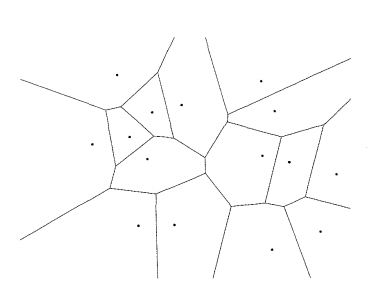
\includegraphics[scale = 0.6]{knn_voronoi_set.png}}
\end{minipage}
\caption{\footnotesize{\textbf{Varona partition of K-NN rules \citep{devroye2013probabilistic}. }}}
\label{fig: knn_voronoi_set}
\end{figure}

\item \begin{remark} (\emph{\textbf{Ordered Statistic}})\\
We fix $x \in \bR^d$, and \emph{\textbf{reorder}} the data $(X_1, Y_1) \xdotx{,} (X_n , Y_n)$ according to \emph{\textbf{increasing values}} of $d(x, X_i)$. The \emph{reordered data sequence} is denoted by
\begin{align*}
(X_{(1)}(x), Y_{(1)}(x)) \xdotx{,} (X_{(n)}(x), Y_{(n)}(x)) 
\end{align*} where $X_{(k)}(x)$ is the $k$-th nearest neighbor of $x$. For short, we write it as $(X_{(k)}, Y_{(k)})$.
\end{remark}

\item \begin{remark} (\emph{\textbf{Efficient Learning Without Hypothesis Class}}) \citep{shalev2014understanding}\\
Note that, in contrast with the algorithmic paradigms that we have discussed so far, like \emph{ERM}, \emph{SRM}, \emph{MDL}, or \emph{RLM}, that are determined by some hypothesis class, $\cH$, \emph{the Nearest Neighbor} method figures out a label \emph{on any test point} \emph{\textbf{without searching for a predictor} \textbf{within some predefined class of functions}}.
\end{remark}
\end{itemize}


\section{Asymptotic Analysis}
\subsection{Consistency of K-Nearest Neighbor Statistics}
\begin{itemize}
\item \begin{definition}
Denote \emph{the probability measure} for $X$ by $\cP_{X}$ and let $B_{x, \epsilon}$ be the \emph{\textbf{closed ball}} centered at $x$ of radius $\epsilon > 0$. The collection of all $x$ with $\cP_{X}(B_{x ,\epsilon}) > 0$ \emph{for all} $\epsilon > 0$ is called \emph{\textbf{the support} of $X$} or $\cP_{X}$.
\end{definition}

\item \begin{lemma}\citep{devroye2013probabilistic}\\
If $x \in \text{support}(\cP_{X})$ and $\lim\limits_{n\rightarrow \infty}k/n = 0$, then 
\begin{align*}
d(x,X_{(k)}(x)) \rightarrow 0, \quad a.s.
\end{align*} 
If $X$ is independent of the data and has probability measure $\cP_{X}$, then 
\begin{align*}
d(X, X_{(k)}(x)) \rightarrow 0, \quad a.s.
\end{align*}   whenever $k/n \rightarrow 0$.
\end{lemma}
\end{itemize}

\subsection{Stone's Lemma and Function of K-Nearest Neighbor}
\begin{itemize}
\item 
\begin{lemma} (\textbf{Stone's Lemma})  \citep{devroye2013probabilistic}\\
For any integrable function $f$, any $n$, and any $k \le n$:
\begin{align}
\sum_{i=1}^{k}\E{}{\abs{f\paren{X_{(i)}(X)}}} &\le k \gamma_d \E{}{\abs{f(X)}}, \label{eqn: stone_lemma}
\end{align}
where $\gamma_d \le \paren{1+ 2/\sqrt{2 - \sqrt{3}}}^d - 1$ depends upon the \textbf{dimension} only.
\end{lemma}

\item \begin{lemma} (\textbf{Approximation with K-NN})  \citep{devroye2013probabilistic}\\
For any integrable function $f$,
\begin{align*}
\frac{1}{k}\sum_{i=1}^{k}\E{}{\abs{f(X) - f\paren{X_{(i)}(X)}}} \to 0
\end{align*} as $n \rightarrow \infty$ whenever $k/n \rightarrow 0$.
\end{lemma}
\end{itemize}

%\subsection{The Asymptotic Probability of Error}

\subsection{Stone's Theorem and Universal Consistency of $k$-NN Rules}
\begin{itemize}
\item \begin{remark} (\emph{\textbf{Estimate Posterior Conditional Probability with Weighted Averages}})\\
Consider a rule based on an estimate of the a \emph{\textbf{posteriori probability}} $\eta$ of the form
\begin{align*}
\eta_n(x) &= \sum_{i=1}^{n}\ind{Y_i = 1}W_{n,i}(x) = \sum_{i=1}^{n}Y_i \,W_{n,i}(x)
\end{align*}
where the weights $W_{n,i}(x) = W_{n,i}(x, X_1 \xdotx{,} X_n)$ are nonnegative and sum to one:
\begin{align*}
\sum_{i=1}^{n}W_{n,i}(x)  = 1.
\end{align*} $\eta_n$ is a \underline{\emph{\textbf{weighted average estimator}}} of $\eta$. 

The \emph{\textbf{classification rule}} is defined as
\begin{align*}
g_n(x) &= \left\{\begin{array}{cc}
0 &  \sum_{i=1}^{n}\ind{Y_i = 1}W_{n,i}(x)  \le \sum_{i=1}^{n}\ind{Y_i = 0}W_{n,i}(x)  \\
1 & \text{o.w.}
\end{array}
\right. \\
&=  \left\{\begin{array}{cc}
0 &   \sum_{i=1}^{n}Y_i \,W_{n,i}(x) \le \frac{1}{2}  \\
1 & \text{o.w.}
\end{array}
\right.
\end{align*}
\end{remark}

\item \begin{remark}
It is intuitively clear that pairs $(X_i, Y_i)$ such that $X_i$ is \emph{close} to $x$ should provide \emph{more information} about $\eta(x)$ than those far from $x$. Thus, the weights are typically \emph{much larger in the neighborhood of $X$}, so $\eta_n$ is roughly \emph{a \textbf{(weighted) relative frequency} of the $X_i$'s} that have label $1$ among points in the neighborhood of $X$. Thus, $\eta_n$ might be viewed as a \emph{\textbf{\underline{local average estimator}}}, and $g_n$ a \emph{\textbf{\underline{local (weighted) majority vote}}}.
\end{remark}

\item \begin{theorem} (\textbf{Stone's Theorem, Universal Consistency of Local Average Estimator}) \citep{devroye2013probabilistic}\\
Assume that for \textbf{any distribution} of $X$, the \textbf{weights} satisfy the following \textbf{three conditions}:
\begin{enumerate}
\item There is a constant $c$ such that, for every \textbf{nonnegative} measurable function $f$ satisfying $\E{}{f(X)} < \infty$,
\begin{align*}
\E{}{\sum_{i=1}^{n}W_{n,i}(X)\,f(X_i)} \le c\E{}{f(X)}.
\end{align*}

\item For all $a > 0$,
\begin{align*}
\lim\limits_{n\rightarrow \infty}\E{}{\sum_{i=1}^{n}W_{n,i}(X)\,\ind{d(X, X_i) > a}} = 0
\end{align*}

\item 
\begin{align*}
\lim\limits_{n\rightarrow \infty}\E{}{\max_{1 \le i \le n}W_{n,i}(X)} = 0.
\end{align*}
\end{enumerate}
Then $g_n$ is \textbf{universally consistent}.
\end{theorem}

\item \begin{remark}
\begin{enumerate}
\item Condition (1) is technical.

\item Condition (2) requires that \emph{\textbf{the overall weight}} of $X_i$'s \emph{\textbf{outside} of any \textbf{ball} of a fixed radius \textbf{centered at $X$}} must go to zero. In other words, \emph{only points in a \textbf{shrinking neighborhood} of $X$ should be taken into account in the \textbf{averaging}}.

\item Condition (3) requires that \emph{\textbf{no single} $X_i$ has \textbf{too large} a contribution to the estimate}.
Hence, \emph{the \textbf{number of points} encountered in the \textbf{averaging} must tend to \textbf{infinity}}.
\end{enumerate}
\end{remark}
\end{itemize}

\section{Non-Asymptotic Analysis}
\subsection{A Generalization Bound for the $k$-NN Rule}
\begin{itemize}
\item 
\begin{lemma} (\textbf{Lipschitz Bayes Classifier Case}) \citep{shalev2014understanding}\\
Let $\cX = [0,1]^d$, $\cY = \set{0,1}$, and $\cP$ be a distribution over $\cX \times \cY$ for which \textbf{the conditional probability function}, $\eta$, is a \textbf{$c$-Lipschitz function}. Let $\cD_m = \set{(X_1, Y_1) \xdotx{,} (X_m, Y_m)}$ be an i.i.d. sample and let $g_{m}$ be its corresponding $1$-NN hypothesis. Let $g^{*}$ be the \textbf{Bayes optimal rule} for $\eta$. Then,
\begin{align*}
\E{\cD_m}{L(g_{m})} &\le 2 L(g^{*}) + c\,\E{X, \cD_m}{\norm{X - X_{(1)}(X)}{}}
\end{align*}
\end{lemma}

\item \begin{lemma} (\textbf{Nearest Neighbor Distance Bound}) \citep{shalev2014understanding}\\
Let $C_1 \xdotx{,} C_r$ be a collection of subsets of some domain set, $\cX$ . Let $\cD$ be a sequence of $m$ points sampled i.i.d. according to some probability distribution, $\cP$ over $\cX$. Then,
\begin{align*}
\E{\cD_m}{\sum_{i: C_i \cap \cD_m = \emptyset}\cP\set{C_i}} \le \frac{r}{e\,m}
\end{align*}
\end{lemma}

\item \begin{proposition} (\textbf{Generalization Bounds for 1-NN Rule}) \citep{shalev2014understanding}\\
Let $\cX = [0,1]^d$, $\cY = \set{0,1}$, and $\cP$ be a distribution over $\cX \times \cY$ for which \textbf{the conditional probability function}, $\eta$, is a \textbf{$c$-Lipschitz function}.  Let $g_m$ denote the result of applying the $1$-NN rule to a sample $\cD_m \sim \cP^{m}$. Then,
\begin{align*}
\E{\cD_m}{L(g_{m})} &\le 2 L(g^{*}) + 4\,c\,\sqrt{d}\,m^{-\frac{1}{d+1}}
\end{align*}
\end{proposition}

\item \begin{proposition} (\textbf{Generalization Bounds for $k$-NN Rule}) \citep{shalev2014understanding}\\
Let $\cX = [0,1]^d$, $\cY = \set{0,1}$, and $\cP$ be a distribution over $\cX \times \cY$ for which \textbf{the conditional probability function}, $\eta$, is a \textbf{$c$-Lipschitz function}.  Let $g_m$ denote the result of applying the $k$-NN rule to a sample $\cD_m \sim \cP^{m}$ where $k \ge 10$. Let $g^{*}$ be the \textbf{Bayes optimal rule} for $\eta$. 
\begin{align*}
\E{\cD_m}{L(g_{m})} &\le \paren{1+ \sqrt{\frac{8}{k}}} L(g^{*}) + (6\,c\,\sqrt{d}+ k)\,m^{-\frac{1}{d+1}}.
\end{align*}
\end{proposition}

\item \begin{remark}  
The theorem implies that if we first fix the data-generating distribution and then \emph{let $m$ go to infinity}, then the error of the $1$-NN rule converges to \emph{twice} the \emph{Bayes error}. The analysis can be generalized to larger values of $k$, showing that the expected error of the $k$-NN rule converges to $\paren{1+ \sqrt{8/k}}$ times the error of the Bayes classifier.  So when $m \rightarrow \infty$ and $k\rightarrow \infty$ with $k/m \rightarrow 0$, we have universal consistency result.
\end{remark}
\end{itemize}

\subsection{The ``Curse of Dimensionality"}
\begin{itemize}
\item \begin{remark} (\emph{\textbf{Sample Complexity Exponentially Growth with Dimensionality}})\\
The upper bound given above grows with $c$ (the Lipschitz coefficient of $\eta$) and with \emph{$d$, the Euclidean dimension of the domain set $\cX$}. In fact, it is easy to see that a necessary condition for the last term to be smaller than  $\epsilon$ is that
\begin{align*}
m \ge \paren{\frac{4\,c\sqrt{d}}{\epsilon}}^{d+1}.
\end{align*}
That is, \emph{the \textbf{size} of the training set \textbf{should increase exponentially with the dimension}}.
\end{remark}

\item \begin{proposition} \citep{shalev2014understanding}\\
For any $c > 1$, and every learning rule, $L$, there exists a distribution over $[0,1]^d \times \set{0,1}$, such that $\eta(x)$ is $c$-Lipschitz, the Bayes error of the distribution is $0$, but for sample sizes $m \le (c + 1)^d/2$, the true error of the rule $L$ is greater than $1/4$.
\end{proposition}

\item \begin{remark}  (\textbf{\emph{The Curse of Dimensionality}})\\
\emph{The \textbf{exponential dependence on the dimension}} is known as \underline{\emph{\textbf{the curse of dimensionality}}}. 

As we saw, the $1$-NN rule might fail if the number of examples is smaller than $\Omega((c + 1)^d)$. Therefore, while the $1$-NN rule does not restrict itself to a predefined set of hypotheses, \emph{it still relies on some \textbf{prior knowledge}} since its success depends on \emph{the \textbf{assumption} that the \textbf{dimension} and \textbf{the Lipschitz constant} of the underlying distribution, $\eta$, are \textbf{not too high}}.
\end{remark}

\end{itemize}
\newpage
\bibliographystyle{plainnat}
\bibliography{reference.bib}
\end{document}